\documentclass
[handout]
{beamer}

%%
%%
%%
% From http://tex.stackexchange.com/questions/2072/beamer-navigation-circles-without-subsections
% Solution #2 or 3:
% \usepackage{etoolbox}
% \makeatletter
% % replace the subsection number test with a test that always returns true
% \patchcmd{\slideentry}{\ifnum#2>0}{\ifnum2>0}{}{\@error{unable to patch}}%
% \makeatother
% Solution #1:
\usepackage{remreset}% tiny package containing just the \@removefromreset command
\makeatletter
\@removefromreset{subsection}{section}
\makeatother
\setcounter{subsection}{1}


\usepackage{etex}
\usepackage{pgf}
\usepackage{tikz}
\usepackage{url}
\usepackage{amsmath}
\usepackage{color}
% \definecolor{red}{rgb}{1,0,0}
\usepackage{ulem}
% \usepackage{booktabs}
\usepackage{colortbl,booktabs}
\renewcommand*{\thefootnote}{\fnsymbol{footnote}}
\usepackage{fancybox}
\usepackage[framemethod=TikZ]{mdframed}
\mdfdefinestyle{FactStyle}{%
  outerlinewidth=0.5,
  roundcorner=1pt,
  leftmargin=1cm,
  linecolor=blue,
  outerlinecolor=blue!70!black,
  backgroundcolor=yellow!40
}
\usepackage{cancel}

  \newcommand\Warning{%
    \makebox[2.4em][c]{%
      \makebox[0pt][c]{\raisebox{.2em}{\Large!}}%
      \makebox[0pt][c]{\color{red}\Huge$\bigtriangleup$}}}%

\usepackage{stackengine}
\usepackage{scalerel}
\usepackage{xcolor}
  \newcommand\dangersign[1][2ex]{%
    \renewcommand\stacktype{L}%
    \scaleto{\stackon[1.3pt]{\color{red}$\triangle$}{\tiny !}}{#1}%
  }



\usepackage{dcolumn}
\newcolumntype{d}[1]{D{.}{.}{#1}}

% From
% http://tex.stackexchange.com/questions/109900/how-can-i-box-multiple-aligned-equations
\usepackage{empheq}
\usepackage{tcolorbox}  \newtcbox{\othermathbox}[1][]{%
  nobeforeafter, tcbox raise base, 
  colback=black!10, colframe=red!30, 
  left=1em, top=0.5em, right=1em, bottom=0.5em}

\newcommand\blue{\color{blue}}
\newcommand\red{\color{red}}
\newcommand\green{\color{green!75!black}}
\newcommand\purple{\color{purple}}
\newcommand\bluegreen{\color{blue!75!green}}
\newcommand\orange{\color{orange}}
\newcommand\redgreen{\color{red!50!green}}
\newcommand\grey{\color{black}}
\newcommand\gap{\vspace{.1in}}
\newcommand\nb{${\red\bullet}\ $}
\newcommand\halfgap{\vspace{.05in}}
\newcommand\divideline{\line(1,0){352}}
\usepackage{marvosym} % for \Smiley

\newcommand{\bluealert}[1]{{\blue\textbf{#1}}}

% \usepackage{beamerthemesplit} %Key package for beamer
\usetheme{Singapore}
% \usetheme{Szeged}
% \usetheme{Garfield}
% \usetheme{CambridgeUS}
% \usenavigationsymbolstemplate{} %Gets rid of slide navigation symbols


\setbeamercolor{separation line}{use=structure,bg=structure.fg!50!bg}
% \begin{beamercolorbox}[colsep=0.5pt]
%   {upper separation line foot}
% \end{beamercolorbox}



\makeatletter
\setbeamertemplate{footline}
{
  \leavevmode%
  \hbox{%
% \begin{beamercolorbox}[colsep=0.5pt]
%   {upper separation line foot}
% \end{beamercolorbox}


  \begin{beamercolorbox}[wd=.5\paperwidth,ht=2.25ex,dp=2ex,colsep=0.5pt]%
    {upper separation line foot}
    \usebeamerfont{author in head/foot}%
    \hspace*{2ex}\insertshortdate:\ \insertshorttitle
  \end{beamercolorbox}%
  \begin{beamercolorbox}[wd=.5\paperwidth,ht=2.25ex,dp=2ex,right]{title in head/foot}%
    \usebeamerfont{title in head/foot}
    {\insertshortauthor}\hspace*{2ex}
  \end{beamercolorbox}}%
  % \begin{beamercolorbox}[wd=.333333\paperwidth,ht=2.25ex,dp=2ex,right]{date in head/foot}%
  %   \usebeamerfont{date in head/foot}\insertshortdate{}\hspace*{2em}
  %   \insertframenumber{} / \inserttotalframenumber\hspace*{2ex} 
  % \end{beamercolorbox}%
  \vskip0pt%
}
\makeatother

\usetikzlibrary{decorations.markings}
\usetikzlibrary{arrows}


\title{Final Exam Review}
\author{Peter Garfield, UCSB Mathematics}
\date{March 15, 2017}
%\institute{}


\useinnertheme{default}

\usefonttheme{serif}
% \usecolortheme{rose}
% \usecolortheme{whale}
% \usecolortheme{orchid}
\usecolortheme{crane}
% \usecolortheme{dolphin}


%TEMPLATE
\setbeamertemplate{navigation symbols}{}

\setbeamertemplate{note page}[compress]

\setbeamertemplate{frametitle}{
  \vspace{0.5em}
  % \begin{centering}
  {\huge\blue\textbf{\textmd{\insertframetitle}}}
  \par
  % \end{centering}
}

% From http://tex.stackexchange.com/questions/7032/good-way-to-make-textcircled-numbers:
\newcommand*\circled[1]{\tikz[baseline=(char.base)]{\node[shape=circle,draw,fill=orange,inner sep=1pt] (char) {#1};}} 
% \renewcommand{\labelenumi}{\circled{\textbf{\arabic{enumi}}}}

\let\olddescription\description
\let\oldenddescription\enddescription
\usepackage{enumitem}
\let\description\olddescription
\let\enddescription\oldenddescription

% \usepackage[loadonly]{enumitem}
\setlist[enumerate,1]{label=\colorbox{orange}{\arabic*.},font=\bfseries}
%\setlist[enumerate,2]{label=\colorbox{blue!25}{(\alph*)},font=\bfseries}
% \setlist[enumerate,1]{label=\arabic*.,font=\bfseries}
\setlist[itemize,1]{label=\red$\bullet$}
\setlist[itemize,2]{label=\blue$\bullet$}

\newcommand\answer[1]{\fbox{#1}}
% \renewcommand\answer[1]{}

\newcommand{\antilog}{\operatorname{antilog}}








\title{Calculus Intro}
\author{Trevor Klar, UCSB Mathematics}
\date{July 19, 2022}



\begin{document}
\small
\renewcommand{\fbox}{}



\frame{
  \frametitle{}
  {\Huge{}Welcome To Math 34A!}\\[.5em]

  {\Huge{}Differential Calculus}
  \vfill
  {\Large{}Instructor:}\\
  \ \hspace*{0.2in} Trevor Klar, \url{trevorklar@math.ucsb.edu}\\
  \ \hspace*{0.2in} South Hall 6431X (Grad Tower, 6th floor, blue side, first door on the right)
  \\[0.5em]

  {\Large{}Office Hours:}\\
  \ \hspace*{0.2in} MTWR after class 2:00-3:00, and by appointment. Details on Gauchospace. 
  \bigskip

  {\tiny \copyright\ 2017-22\ Daryl Cooper, Peter Garfield, Ebrahim Ebrahim, Nathan Schley, and Trevor Klar}\\
  Please do not distribute outside of this course.
  \vfill

}


\section*{Review}


\frame{
A nice thing about derivatives...
\begin{align*}  
\frac{d}{dx} ( a\cdot f(x) + b\cdot g(x) ) 
&= a\frac{d}{dx}f(x) + b\frac{d}{dx} g(x)\\[0.75em]
&= a\cdot f'(x)+b\cdot g'(x)
\end{align*}
For example...
\pause
$$
\begin{array}{lclcl}
 \frac{d}{dx} ( 3x^2+ 5x ) &=& 3  \frac{d}{dx} x^2 &+ & 5 \frac{d}{dx}x\\[0.75em]
                           &=& 3(2x)               &+  & 5(1)\\[0.75em]
                           &=& 6x                  &+ & 5
\end{array}
$$
}


\frame{
  \frametitle{A Warning!}

  \begin{empheq}[box=\othermathbox]{align*}
    \ \hfill \raisebox{-0.5em}{\dangersign[6ex]} \hspace*{0.2in}
    \frac{d}{dx}\left(f(x)g(x)\right) {\red\ne} f'(x) \times g'(x)
    \hspace*{0.2in} \raisebox{-0.5em}{\dangersign[6ex]} \hfill \ 
  \end{empheq}
  \pause
  \bigskip

  \alert{Example:} \quad 
  $5x^4
  = \dfrac{d}{dx}\left(x^5\right)
  = \dfrac{d}{dx}\left(x^2\cdot x^3\right)
  {\red\ne}(2x)(3x^2)
  =6x^3$
  \bigskip
  \pause

  \alert{Example:} Find the derivative of $(x+1)(2x+3)$
  \bigskip
  \pause

  \alert{Question:}\ $\displaystyle\frac{d}{dx}\left((x^2+1)(x^3+1)\right)=$?
  \begin{center}
    A$=6x^3$
    \quad 
    B$ = 5x^4+3x^2+2x$
    \quad 
    C$ = x^5+x^3+x^2+1$
    \quad 
    D$ = \text{Other}$
  \end{center}
  \bigskip
  \pause

  \alert{Answer:}\ \fbox{B}

  \vspace*{2in}

}



\frame{
  \frametitle{Review Examples:}

  {\red(1)}\ What is the $x$-coordinate of the point on the graph of
  $y=4x^2-3x+7$ where the graph has slope $13$? 
  \begin{center}
    A$=0$
    \quad 
    B$=1$
    \quad 
    C$=2$
    \quad 
    D$=3$
    \quad 
    E$=4$
    \pause
    \quad
    \fbox{C}
  \end{center}
  \bigskip

  {\red(2)}\ A circle is expanding so that after $R$ seconds it has
  radius $R$ cm.  What is the rate of increase of area inside the
  circle after $2$ seconds?
  \begin{center}
    A$=4\pi$
    \quad 
    B$ = 2\pi R^2$
    \quad 
    C$ =2$
    \quad 
    D$ = 2\pi R$
    \quad 
    E$ = \pi R^2$
    \pause
    \quad
    \fbox{A}
  \end{center}
  \bigskip

  % \gap $A(R)=$ area inside circle of radius $R$\\
  % {\red rate of increase of area
  %   = derivative}
  % = $\frac{d}{dR}\left(\pi R^2\right)=2\pi R$\hfill{\green explain}\pause\\
  % So rate of increase of area when $R=2$ is $2\pi(2)=4\pi$
  % 
  % \includegraphics[scale=0.5]{circlefirstordera.pdf}

}



%----

\frame{
  \frametitle{Differentiating $f(x) = e^{kx}$}

  \begin{minipage}[b]{0.35\linewidth}
    \begin{empheq}[box=\othermathbox]{align*}
      \frac{d}{dx}\left(e^{{\red k}x}\right) 
      & = {\red k}e^{{\red k}x}
    \end{empheq}
  \end{minipage}
  \hspace*{0.2in}
  versus
  \hspace*{0.2in}
  \begin{minipage}[b]{0.35\linewidth}
    \begin{empheq}[box=\othermathbox]{align*}
      \frac{d}{dx}\left(x^{{\red n}}\right) 
      & = {\red n} x^{{\red n}-1}
    \end{empheq}
  \end{minipage}
  \bigskip

  \begin{empheq}[box=\othermathbox]{align*}
    \raisebox{-0.5em}{\dangersign[6ex]}  
    \hspace*{0.1in}
    \text{Do not get confused and write}\ 
    \dfrac{d}{dx} \big( e^{{\red k}x} \big) = {\red k}e^{({\red k}-1)x}.
    \hspace*{0.1in}
    \raisebox{-0.5em}{\dangersign[6ex]}  
  \end{empheq}
  \bigskip

  \alert{Question:}\ Find $\dfrac{d}{dx}\left( 4e^{3x}+ 5x^3\right)$
  \begin{center}
    A$=12e^{2x}+15x^2$
    \qquad 
    B$ = 12e^{3x}+15 x^3$
    \qquad 
    C$ = 4e^{3x}+15x^2$
    \\
    \ 
    \quad 
    D$=12e^{3x}+15x^2$
    \quad
    E$= \text{Other}$
    \pause
    \quad
    \fbox{D}
  \end{center}

}





\frame{
  \frametitle{Example}

  \begin{empheq}[box=\othermathbox]{align*}
    \frac{d}{dx}\left(e^{{\red k}x}\right) 
    & = {\red k}e^{{\red k}x}
  \end{empheq}

  The temperature (in ${}^{\circ}\,\text{C}$) of a cup of coffee $t$
  hours after it is made is $f(t)=50+40e^{-2t}$. 
  \smallskip

  {\red(a)}\ What is the {\red initial} temperature when the coffee is made?
  \begin{center}
    A$ = 40$
    \quad 
    B$ = 50$
    \quad 
    C$ = 90$
    \quad 
    D$ = 100$
    \pause
    \quad
    \fbox{C}
  \end{center}
  \gap

  {\red(b)} How quickly is the coffee {\blue cooling down} initially?
  This means how many degrees per hour is the temperature {\blue going
    down} instantaneously at $t=0$? 
  \begin{center}
    A$ = 20$
    \quad 
    B$ = 40$
    \quad 
    C$ = 60$
    \quad 
    D$ = 80$
    \quad 
    E$ =100$
    \pause
    \quad
    \fbox{D}
  \end{center}
  \gap


}



\frame{
  \frametitle{More Examples}

  \begin{empheq}[box=\othermathbox]{align*}
    \frac{d}{dx}\left(e^{{\red k}x}\right) 
    & = {\red k}e^{{\red k}x}
  \end{empheq}

  {\red(1)}\ $\displaystyle\frac{d}{dx}\left(\frac{3}{e^{2x}}\right)=$?
  \begin{center}
    A $= \frac{3}{2e^{2x}}$
    \quad 
    B $= \frac{3}{2e^{x}}$
    \quad 
    C $= \frac{6}{e^{2x}}$
    \quad 
    D $= \frac{-6}{e^{2x}}$
    \pause
    \quad
    \fbox{D}    
  \end{center}
  \gap

  {\red(2)}\ The number of grams of {\blue
    Einsteinium-253} %\footnote{\red half-life is $20.47$ days}
  after $t$ days is $m(t)=10e^{-t/30}$.  How quickly is the mass
  changing (in grams per day) when $t=0$?
  \begin{center}
    A $= -1/30$
    \quad 
    B $= -1/3$
    \quad 
    C $= -10e^{-t/30}$
    \quad 
    D $= -\frac{1}{3}\,e^{t/30}$
    \pause
    \quad
    \fbox{B}
  \end{center}



}


%-------------------------




\section{Higher Derivatives}

\frame{
  \frametitle{\S8.12: The Second Derivative}

  \alert{Today:}\ We can take the derivative of a function repeatedly!
  \bigskip

  \alert{Example:}\ If $f(x)=x^3-3x+2$, then
  \begin{itemize}
  \item[\nb] $\dfrac{df}{dx}={\blue f'(x)}= $ \pause ${\blue 3x^2-3}$
    \smallskip

  \item[\nb] The {\red second derivative} of $f(x)$ is $\displaystyle
      \frac{d}{dx}\left(\frac{df}{dx}\right)
      = {\red f''(x)}
      = 
      \pause 
      {\red 6x}$.
    \pause\newline
    This is written $f''(x)$ or $\dfrac{d^2f}{dx^2}$.
    \pause

  \item[\nb] The {\red
      third derivative} of $f(x)$ is $\displaystyle
      \frac{d}{dx}\left(\frac{d^2f}{dx^2}\right)
      = {\red f'''(x)}
      = 
      \pause 
      {\red 6}$.
    \pause\newline
    This is written $f'''(x)$ or $\dfrac{d^3f}{dx^3}$.
    \pause

  \item[\nb] {\blue Keep Going!}\ \ \pause 
    The {\red fourth derivative}\ is $\dfrac{d^4f}{dx^4} = f''''(x) =
    0$. 
    \pause

  \item[\nb]
    The fun ends here, for this $f(x)$ all {\red higher derivatives} are zero.
  \end{itemize}

}

\frame{
  \frametitle{Examples}

  General idea: Differentiating the function ${\red n}$ times gives us
  the {\blue ${\red n}$th derivative} of $f$.  
  It is written as
  \begin{equation*}
    {{f'''}^{\cdots}}{}''''(x) 
    = f^{(n)}(x)
    = \frac{d^nf}{dx^n}.
  \end{equation*}
  \bigskip
  \pause

  {\red(1)}\ What is the second derivative of $3x^2-5x+7$?
  \begin{center}
    A$=0$
    \quad 
    B$ = 7$
    \quad 
    C$ = 6$
    \quad 
    D$ = 3$
    \quad 
    E$ = -5$
    \pause
    \quad
    \fbox{C}
  \end{center}
  \bigskip
  \pause

  {\red(2)}\ $\dfrac{d^2}{dx^2}\left(x^5\right)=$?
  \begin{center}
    A$ = 20$
    \quad 
    B$ = 5x^4$
    \quad 
    C$ = 0$
    \quad 
    D$ = 20x^4$
    \quad 
    E$ = 20x^3$
    \pause
    \quad
    \fbox{E}
  \end{center}
  \bigskip
  \pause

  {\red(3)}\ $\dfrac{d^2}{dx^2}\left(\sqrt{x}\right)=$?
  \begin{center}
    A$ = \frac{1}{4}x^{-3/2}$
    \quad 
    B$ = \frac{-1}{4}x^{-1/2}$
    \quad 
    C$ = \frac{-1}{4}x^{-3/2}$ 
    \quad 
    D$ = \frac{1}{2}x^{-1/2}$
    \quad 
    E$ = 0$
    \pause
    \ 
    \fbox{C}
  \end{center}

}



\frame{
  \frametitle{More Examples}

  {\red(4)}\ $\dfrac{d^2}{dt^2}\left(e^{{\red 3}t}\right)=$?
  \begin{center}
    A$ = e^{3t}$
    \quad 
    B$ = 3e^{2t}$
    \quad 
    C$ = 9e^{3t}$
    \quad 
    D$ = 3e^{3t}$
    \quad 
    E$ = 9e^t$
    \pause
    \qquad
    \fbox{C}
  \end{center}
  \gap 

  {\red(5)} Find $f{\red '''}(x)$ when $f(x)=x^3$.
  \begin{center}
    A$=  6x^2$
    \quad 
    B$ = 0$
    \quad 
    C$ = 3x$
    \quad 
    D$ = 3x^2$
    \quad 
    E$ = 6$
    \pause
    \quad
    \fbox{E}
  \end{center}
  \bigskip

  {\red(6)}\ If $f(x)= x^3-4x^2 + 7x -31$, then $f{\red ''}(10)=$? 
  \begin{center}
    A$ = 6$
    \quad 
    B$ = 3x^2-8x$
    \quad 
    C$ = 6x$
    \quad 
    D$ = 60$
    \quad 
    E$ = 52$
    \pause
    \quad
    \fbox{E}
  \end{center}
  \bigskip


}


\section{Acceleration}

\frame{
  \frametitle{Example: Acceleration}

  The {\red acceleration}\ due to gravity is
  \begin{equation*}
    32\ \text{{\blue feet per second per second}}
      = 32\ \text{ft}/\text{sec}^2. 
  \end{equation*}
  \vspace*{-1em}

  \uncover<2->{%
    \bluealert{This means:}
    \begin{center}
      \begin{mdframed}[style=FactStyle]
        every second you fall, \\
        your speed increases by $32\ \text{ft}/\text{sec}$
        \uncover<3->{$\approx 22\ \text{mph}$.}
        % \vspace*{-1em}
      \end{mdframed}
    \end{center}
  }
  \begin{align*}
    \uncover<4->{%
    \text{{\red acceleration}}
    & = \text{{\orange rate of change}\ of {\blue velocity}} 
    & = \text{{\orange derivative} of {\blue velocity}}.\\
    }
    \uncover<5->{%
    \text{{\blue velocity}}
    & = \text{{\orange rate of change} of {\purple distance}}
    & = \text{{\orange derivative} of {\purple distance}}.
      }
  \end{align*}

  \uncover<6->{%
    Therefore
    \begin{center}
      \begin{mdframed}[style=FactStyle]
        \vspace*{-0.5em}
        \begin{equation*}
          \text{{\red acceleration}}
          = \text{second derivative of {\purple distance}}
        \end{equation*}
      \end{mdframed}
    \end{center}
  }

  \uncover<7->{%
    \alert{Example:}\ Height of ball is $h(t)=20t-5t^2$\ meters after $t$ seconds.\\
    {\red (a)}\ {\blue Velocity}\ of ball after $t$ seconds is\ 
  }
  \uncover<8->{$h{\red '}(t)=20-10t\ \text{m}/\text{sec}$}\\
  \uncover<9->{%
    {\red (b)}\ {\red Acceleration}\ of ball after $t$ seconds is\ 
  }
  \uncover<10->{$h{\red''}(t)=-10\ \text{m}/\text{sec}^2$}

  % \gap $\purple -$ sign because UP is positive in this problem and gravity accelerates DOWN so acceleration is {\purple negative}

}

\frame{
  \frametitle{It's not the speed that kills}
  % \includegraphics[scale=0.7]{speedkills.pdf}
  % \gap 

  Suppose you hit a brick wall at $60$ mph.
  \pause

  \alert{Question:}\ What is your (sudden!) acceleration?
  \pause

  \begin{align*}
    \left( \ \parbox{1.08in}{%
    \ Average rate of\ \\
    change of velocity\\
    \hspace*{0.2in}in stopping 
    }\ 
    \right)
    & = \frac{\Delta\ \text{velocity}}{\Delta\ \text{time}}
      = \frac{-60\ \text{mph}}{1/10\ \text{sec}} \\
    & \approx \frac{-88\ \text{ft}/\text{sec}}{1/10\ \text{sec}}
      = -880\ \text{ft}/\text{sec}^2.
  \end{align*}
  \pause
  Since $1\ \text{gravity} = 32\ \text{ft}/\text{sec}^2$, this is about
  \begin{equation*}
    880\ \text{ft}/\text{sec}^2
    = \left( 880\ \text{ft}/\text{sec}^2 \right)
    \times \frac{1\ \text{gravity}}{32\ \text{ft}/\text{sec}^2}
    \pause
    \approx 28\ \text{``g''}.
  \end{equation*}
  %
  The force at which the brick wall pushes you is {\red{}28}
  times your weight.
  \pause

  If you weigh $110$ pounds, this force is about $\text{\red $3000$\ pounds}
  = \text{\red $1.5$\ tons}$.

}


\frame{
  \frametitle{A Rocket}

  A rocket is fired vertically upwards.  The height after $t$ seconds
  is $2t^3+5t^2$ meters.
  \smallskip

  \alert{Question:}\ What is the acceleration in
  $\text{m}/\text{sec}^2$ after $t$ seconds? 
  \begin{center}
    A$=2t^3+5t^2$
    \quad 
    B$=6t^2+10t$
    \quad 
    C$ = 12t+10$
    \quad 
    D$ = 12$
    \quad 
    E$ = 0$
    \pause
    \quad
    \fbox{C}
  \end{center}
  \medskip
  \pause

  Idea:
  \begin{itemize}
  \item[\nb] $h(t) = \text{height in meters at time $t$ seconds}$ 
    \smallskip

  \item[\nb] $h'(t) = \text{velocity in $\text{m}/\text{sec}$\ at time $t$ seconds}$ 
    \smallskip

  \item[\nb] $h''(t) = \text{acceleration in $\text{m}/\text{sec}^2$\ at time $t$ seconds}$ 
    \bigskip

  \end{itemize}

  \alert{More Questions:}
  \smallskip

  {\red(a)}\ What can we say about $f(t)$ if $f'(t)=0$ for {\red all} $t$?
  \pause
  \smallskip

  {\red(b)}\ What can we say about $f(t)$ if $f''(t)=0$ for {\red all} $t$?
  \pause
  \smallskip

  \vspace*{2in}

}

\section{Concavity}

\frame{
  \frametitle{Application 2: Concavity}

  \begin{align*}
    \frac{df}{dx}
    & = \text{rate of change of $f(x)$}\\[0.5em]
    %
    \text{and so}\ 
    \frac{d^2f}{dx^2}
    & =\frac{d}{dx}\left({\red \frac{df}{dx}}\right)
      = \text{rate of change of $\red\dfrac{df}{dx}$}
  \end{align*}

  \bluealert{Conclusion:}\\[-2em]
  \begin{center}
    \begin{mdframed}[style=FactStyle]
      The second derivative tells you how quickly the {\red rate of
        change} is changing.
    \end{mdframed}
  \end{center}
  \vspace*{-1em}

  \bluealert{Uses of second derivative:}
  \begin{itemize}
  \item[\nb] We've seen: {\blue acceleration} is the rate of change of velocity \\
    So: {\blue acceleration}\ is the second derivative of distance traveled.
    \pause

  \item[\nb] Is the graph {\blue concave up} or {\blue concave down}?
    \pause

  \item[\nb] Are things  {\blue changing for better or worse}?

  \end{itemize}

}

\frame{
  \frametitle{Meanings: The First Derivative}

  \begin{center}
    \begin{tikzpicture}[x=15mm,y=5mm,>=latex]
      \only<1>{%
        \draw[ultra thick,blue,domain=-1:3,smooth] plot (\x,{(\x)^3-3*(\x)^2+2});
      }
      \only<2->{%
        \draw[ultra thick,blue,domain=-1:0,smooth] plot (\x,{(\x)^3-3*(\x)^2+2});
        \draw[ultra thick,red,domain=0:2,smooth] plot (\x,{(\x)^3-3*(\x)^2+2});
        \draw[ultra thick,blue,domain=2:3,smooth] plot (\x,{(\x)^3-3*(\x)^2+2});
        \filldraw[green] (0,2) circle (2pt);
        \filldraw[green] (2,-2) circle (2pt);
      }
      \uncover<3->{%
        \draw[ultra thick,blue,<-] (-1,-2.5) -- (0,-2.5);
        \draw[blue,fill=white] (0,-2.5) circle (2pt);
        \draw[ultra thick,blue,->] (2,-2.5) -- (3,-2.5);
        \draw[blue,fill=white] (2,-2.5) circle (2pt);
        \draw[ultra thick,red] (0,-2.85) -- (2,-2.85);
        \draw[red,fill=white] (0,-2.85) circle (2pt);
        \draw[red,fill=white] (2,-2.85) circle (2pt);
        \node[blue] at (-0.5,-3.5) {$f(x)$ incr};
        \node[red] at (1,-3.5) {$f(x)$\ decr};
        \node[blue] at (2.5,-3.5) {$f(x)$\ incr};
      }
      \uncover<5->{%
        \node[blue] at (-0.5,-4.5) {$f'(x)>0$};
        \node[red] at (1,-4.5) {$f'(x)<0$};
        \node[blue] at (2.5,-4.5) {$f'(x)>0$};
      }
      \begin{scope}
        \clip (-1.5,-4) rectangle (3.5,2.75);
              \uncover<4->{%
        % Tangent lines to $y=x^3-3x^2+2$ has slope $y'=3x^2-6x=3x(x-2)$.
        % \draw[blue,domain=-1:0] plot (\x,{(-5/5)^3-3*(-5/5)^2+2+3*(-5/5)*(-5/5-2)*(\x+5/5)});
        % \draw[blue,domain=-1:0] plot (\x,{(-4/5)^3-3*(-4/5)^2+2+3*(-4/5)*(-4/5-2)*(\x+4/5)});
        % \draw[blue,domain=-1:0] plot (\x,{(-3/5)^3-3*(-3/5)^2+2+3*(-3/5)*(-3/5-2)*(\x+3/5)});
        % \draw[blue,domain=-1:0] plot (\x,{(-2/5)^3-3*(-1/5)^2+2+3*(-2/5)*(-2/5-2)*(\x+2/5)});
        % \draw[blue,domain=-1:0] plot (\x,{(-1/5)^3-3*(-1/5)^2+2+3*(-2/5)*(-1/5-2)*(\x+1/5)});
        % \draw[blue,domain=-1:0] plot (\x,{(-1/3)^3-3*(-1/3)^2+2+3*(-1/3)*(-1/3-2)*(\x+1/3)});
        \draw[thick,blue,domain=-1:0] plot (\x,{(-1/2)^3-3*(-1/2)^2+2+3*(-1/2)*(-1/2-2)*(\x+1/2)});
        \draw[thick,red,domain=0:1.85] plot (\x,{(1)^3-3*(1)^2+2+3*(1)*(1-2)*(\x-1)});
        \draw[thick,blue,domain=2.2:3.5] plot (\x,{(2.5)^3-3*(2.5)^2+2+3*(2.5)*(2.5-2)*(\x-2.5)});
        \fill[black] (-0.5,{(-1/2)^3-3*(-1/2)^2+2}) circle (2pt);
        \fill[black] (1,{(1)^3-3*(1)^2+2}) circle (2pt);
        \fill[black] (2.5,{(2.5)^3-3*(2.5)^2+2}) circle (2pt);
      }
      \end{scope}
    \end{tikzpicture}
  \end{center}
  \bigskip

  \uncover<6->{%
    \bluealert{Point:} 

    \begin{mdframed}[style=FactStyle]
      \vspace*{-1.25em}
      \begin{align*}
        {\blue f'(x) > 0} & \iff\ \text{$f(x)$\ is increasing} \\
        {\red f'(x) < 0} & \iff\ \text{$f(x)$\ is decreasing} 
      \end{align*}
    \end{mdframed}
  }
  \vspace*{3in}

}

\frame{
  \frametitle{Meanings: The Second Derivative}

  \begin{center}
    \begin{tikzpicture}[x=15mm,y=5mm,>=latex]
      \only<1>{%
        \draw[ultra thick,blue,domain=-1:3,smooth] plot (\x,{(\x)^3-3*(\x)^2+2});
      }
      \only<2->{%
        \draw[ultra thick,green!50!black,domain=-1:1,smooth] plot (\x,{(\x)^3-3*(\x)^2+2});
        \draw[ultra thick,orange!90!black,domain=1:3,smooth] plot (\x,{(\x)^3-3*(\x)^2+2});
        \filldraw[blue] (1,0) circle (2pt);
      }
      \uncover<3->{%
        \draw[ultra thick,green!50!black,<-] (-1,-2.5) -- (1,-2.5);
        \draw[green!50!black,fill=white] (1,-2.5) circle (2pt);
        \draw[ultra thick,orange!90!black,->] (1,-2.85) -- (3,-2.85);
        \draw[orange!90!black,fill=white] (1,-2.85) circle (2pt);
        \node[green!50!black] at (0,-3.5) {$f(x)$ cc down};
        \node[orange!90!black] at (2,-3.5) {$f(x)$\ cc up};
      }
      \begin{scope}
        \clip (-1.5,-4) rectangle (3.5,2.75);
              \uncover<4->{%
        % Tangent lines to $y=x^3-3x^2+2$ has slope $y'=3x^2-6x=3x(x-2)$.
        % \draw[blue,domain=-1:0] plot (\x,{(-5/5)^3-3*(-5/5)^2+2+3*(-5/5)*(-5/5-2)*(\x+5/5)});
        % \draw[blue,domain=-1:0] plot (\x,{(-4/5)^3-3*(-4/5)^2+2+3*(-4/5)*(-4/5-2)*(\x+4/5)});
        % \draw[blue,domain=-1:0] plot (\x,{(-3/5)^3-3*(-3/5)^2+2+3*(-3/5)*(-3/5-2)*(\x+3/5)});
        % \draw[blue,domain=-1:0] plot (\x,{(-2/5)^3-3*(-1/5)^2+2+3*(-2/5)*(-2/5-2)*(\x+2/5)});
        % \draw[blue,domain=-1:0] plot (\x,{(-1/5)^3-3*(-1/5)^2+2+3*(-2/5)*(-1/5-2)*(\x+1/5)});
        % \draw[blue,domain=-1:0] plot (\x,{(-1/3)^3-3*(-1/3)^2+2+3*(-1/3)*(-1/3-2)*(\x+1/3)});
        \draw[thick,green!50!black,domain=-1:0] plot (\x,{(-2/3)^3-3*(-2/3)^2+2+3*(-2/3)*(-2/3-2)*(\x+2/3)});
        \draw[thick,green!50!black,domain=-1:0.3333] plot (\x,{(-1/3)^3-3*(-1/3)^2+2+3*(-1/3)*(-1/3-2)*(\x+1/3)});
        \draw[thick,green!50!black] (-0.5,2) -- (0.5,2);
        \draw[thick,green!50!black,domain=-0.3333:1] plot (\x,{(1/3)^3-3*(1/3)^2+2+3*(1/3)*(1/3-2)*(\x-1/3)});
        \draw[thick,green!50!black,domain=0:1] plot (\x,{(2/3)^3-3*(2/3)^2+2+3*(2/3)*(2/3-2)*(\x-2/3)});
        % \draw[thick,red,domain=0:1.85] plot (\x,{(1)^3-3*(1)^2+2+3*(1)*(1-2)*(\x-1)});
        % \draw[thick,blue,domain=2.2:3.5] plot (\x,{(2.5)^3-3*(2.5)^2+2+3*(2.5)*(2.5-2)*(\x-2.5)});
        \fill[black] ({-2/3},{(-2/3)^3-3*(-2/3)^2+2}) circle (2pt);
        \fill[black] ({-1/3},{(-1/3)^3-3*(-1/3)^2+2}) circle (2pt);
        \fill[black] (0,2) circle (2pt);
        \fill[black] ({1/3},{(1/3)^3-3*(1/3)^2+2}) circle (2pt);
        \fill[black] ({2/3},{(2/3)^3-3*(2/3)^2+2}) circle (2pt);
        % \fill[black] (1,{(1)^3-3*(1)^2+2}) circle (2pt);
        % \fill[black] (2.5,{(2.5)^3-3*(2.5)^2+2}) circle (2pt);
      }
      \uncover<6->{%
        \draw[thick,orange!90!black,domain=2.3:3.3] plot (\x,{(8/3)^3-3*(8/3)^2+2+3*(8/3)*(8/3-2)*(\x-8/3)});
        \draw[thick,orange!90!black,domain=1.9:2.9] plot (\x,{(7/3)^3-3*(7/3)^2+2+3*(7/3)*(7/3-2)*(\x-7/3)});
        \draw[thick,orange!90!black] (1.5,-2) -- (2.5,-2);
        \draw[thick,orange!90!black,domain=1.3333:2.1] plot (\x,{(5/3)^3-3*(5/3)^2+2+3*(5/3)*(5/3-2)*(\x-5/3)});
        \draw[thick,orange!90!black,domain=0.5:2] plot (\x,{(4/3)^3-3*(4/3)^2+2+3*(4/3)*(4/3-2)*(\x-4/3)});
        % \draw[thick,red,domain=0:1.85] plot (\x,{(1)^3-3*(1)^2+2+3*(1)*(1-2)*(\x-1)});
        % \draw[thick,blue,domain=2.2:3.5] plot (\x,{(2.5)^3-3*(2.5)^2+2+3*(2.5)*(2.5-2)*(\x-2.5)});
        \fill[black] ({4/3},{(4/3)^3-3*(4/3)^2+2}) circle (2pt);
        \fill[black] ({5/3},{(5/3)^3-3*(5/3)^2+2}) circle (2pt);
        \fill[black] (2,-2) circle (2pt);
        \fill[black] ({7/3},{(7/3)^3-3*(7/3)^2+2}) circle (2pt);
        \fill[black] ({8/3},{(8/3)^3-3*(8/3)^2+2}) circle (2pt);
      }
      \end{scope}
      \uncover<5->{%
        \node[green!50!black] at (0,-4.5) {$f''(x)<0$};
      }
      \uncover<7->{%
        \node[orange!90!black] at (2,-4.5) {$f''(x)>0$};
      }
    \end{tikzpicture}
  \end{center}
  \vspace*{-1em}

  \uncover<8->{%
    \bluealert{Point:} 

    \begin{mdframed}[style=FactStyle]
      \vspace*{-1.25em}
      \begin{align*}
        {\color{orange!90!black}f''(x) > 0} 
        & \iff\ \text{$f'(x)$\ is increasing} \\
        & \iff\ \text{$f(x)$\ is concave up} \\[0.5em]
        {\color{green!50!black}f''(x) < 0}
        & \iff\ \text{$f'(x)$\ is decreasing} \\
        & \iff\ \text{$f(x)$\ is concave down} 
      \end{align*}
    \end{mdframed}
  }
  \vspace*{3in}

}



\frame{
  \frametitle{Concavity}

  \begin{mdframed}[style=FactStyle]
    \vspace*{-1.25em}
    \begin{align*}
      {\color{orange!90!black}f''(x) > 0} & \iff\ \text{$f(x)$\ is concave up} \\
      {\color{green!50!black}f''(x) < 0} & \iff\ \text{$f(x)$\ is concave down} 
    \end{align*}
  \end{mdframed}

  {\red(1)}\ For which values of $x$ is $f(x)=x^3-6x^2+3x+2$ concave up?
  \begin{center}
    A\ when $x=0$
    \quad 
    B\ when $x<6$
    \quad 
    C\ when $x>6$\\
    \ 
    \quad 
    D\ when $x<2$
    \quad 
    E\ when $x>2$
    \quad
    \uncover<2->{\fbox{E}}
  \end{center}

  \uncover<3->{
  {\red(2)}\ Where is $f{\red''}(x)>0$? 

  \
  \hfill
  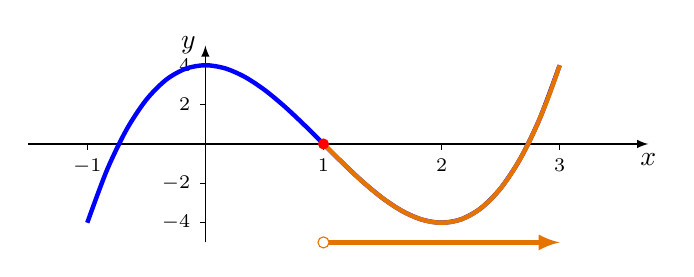
\begin{tikzpicture}[x=15mm,y=2.5mm,>=latex]
    %
    \draw[thin,black,->] (-1.5,0) -- (3.75,0) node[below] {$x$};
    \draw[thin,black,->] (0,-5) -- (0,5) node[left] {$y$};
    % ticks:
    \foreach \x in {-1,1,2,3}
    {
      \draw[thin,black] (\x,0) -- (\x,-2pt) node[below] {$\scriptstyle\x$};
    }
    \foreach \y in {-4,-2,2,4}
    {
      \draw[thin,black] (0,\y) -- (-2pt,\y) node[left] {$\scriptstyle\y$};
    }
    \draw[ultra thick,blue,domain=-1:3,smooth] plot (\x,{2*(\x)^3-6*(\x)^2+4});
    \uncover<4->{%
      \draw[ultra thick,orange!90!black,domain=1:3,smooth] plot (\x,{2*(\x)^3-6*(\x)^2+4});
      \draw[ultra thick,orange!90!black,->] (1,-5) -- (3,-5);
      \draw[orange!90!black,fill=white] (1,-5) circle (2pt);
      \fill[red] (1,0) circle (2pt);
    }
  \end{tikzpicture}
  \hfill
  \ 
  \vspace*{-1em}

  \begin{center}
    A\ when $x<2$
    \quad 
    B\ when $x>2$
    \quad
    C\ when $x<1$\\
    \ 
    \quad 
    D\ when $x>1$
    \quad
    E\ when $-0.7<x<1$
    \pause
    \quad
    \uncover<4->{\fbox{D}}
  \end{center}
}

}











\end{document}


